% thesis_main.tex
% Main LaTeX file for HCMUT Master's Thesis
% Compile this file with XeLaTeX
%
% Author: Nguyễn Tấn Khôi (2171017)
% Advisor: TS. Phạm Việt Cường
% Title: Ứng Dụng Reinforcement Learning Điều Khiển Phân Tán Hệ Đa Robot Tránh Va Chạm
% Institution: ĐH Bách Khoa - ĐHQG TP.HCM
% Date: 2025-12-14
%
% Compilation commands:
%   xelatex thesis_main.tex
%   biber thesis_main
%   xelatex thesis_main.tex
%   xelatex thesis_main.tex
%
% Or simply use: make

\documentclass[a4paper,12pt,oneside,openany]{extbook}

%% ============================================================================
%% Load Preamble (all packages and configurations)
%% ============================================================================

\input{preamble}

%% ============================================================================
%% BEGIN DOCUMENT
%% ============================================================================

\begin{document}

%% ============================================================================
%% FRONT MATTER (Không đánh số trang)
%% ============================================================================

\pagenumbering{gobble}

% Trang bìa (Bìa chính)
% chapters/00_cover.tex
% Trang bìa (có đường viền và logo) for HCMUT Master's Thesis
% Theo mẫu biểu mẫu 10
% Author: Nguyễn Tấn Khôi
% Date: 2025-12-14

%% ============================================================================
%% TRANG BÌA (BÌA CHÍNH) - CÓ ĐƯỜNG VIỀN VÀ LOGO
%% ============================================================================

\begin{titlepage}

% Double border around cover page
\begin{tikzpicture}[remember picture,overlay]
  % Outer border (2pt thick)
  \draw[line width=2pt]
    ([xshift=2cm,yshift=-2cm]current page.north west)
    rectangle
    ([xshift=-1cm,yshift=2cm]current page.south east);

  % Inner border (1pt thick, 3mm inside outer)
  \draw[line width=1pt]
    ([xshift=2.3cm,yshift=-2.3cm]current page.north west)
    rectangle
    ([xshift=-1.3cm,yshift=2.3cm]current page.south east);
\end{tikzpicture}

\begin{center}

% Tên trường
{\fontsize{14}{16}\selectfont
ĐẠI HỌC QUỐC GIA TP. HCM\\
\textbf{TRƯỜNG ĐẠI HỌC BÁCH KHOA}\\[0.3cm]
--------------------
}


% Logo
% 
\includegraphics[width=3cm]{images/bk-logo.png}

\vspace{2cm}

% Họ và tên học viên (in đậm)
{\fontsize{15}{16}\selectfont\bfseries
\MakeUppercase{\authorname}\\
}

\vspace{2cm}

% Tên đề tài (in đậm, cỡ lớn hơn)
{\fontsize{16}{19}\selectfont\bfseries
\MakeUppercase{\thesistitleVN}\\
}

\vspace{1.5cm}

\begin{center}
{\fontsize{13}{15}\selectfont
\begin{tabular}{@{}l l@{}}
Chuyên ngành: & \major \\
Mã số:        & \majorcode \\
\end{tabular}
}
\end{center}

\vspace{2cm}

% LUẬN VĂN THẠC SĨ
{\fontsize{21}{24}\selectfont\bfseries
LUẬN VĂN THẠC SĨ\\
}

\vfill

% Địa điểm và thời gian
{\fontsize{13}{15}\selectfont
TP. HỒ CHÍ MINH, tháng 12 năm 2025\\
}

\end{center}
\end{titlepage}


% Trang 1 (giống trang bìa)
% chapters/00_cover_secondary.tex
% Trang 1 (giống nội dung trang bìa nhưng KHÔNG có viền và logo)
% Theo mẫu biểu mẫu 10
% Author: Nguyễn Tấn Khôi
% Date: 2025-12-14

%% ============================================================================
%% TRANG 1 (KHÔNG CÓ VIỀN VÀ LOGO)
%% ============================================================================

\begin{titlepage}

\begin{center}

% Tên trường
{\fontsize{14}{16}\selectfont
ĐẠI HỌC QUỐC GIA TP. HCM\\
\textbf{TRƯỜNG ĐẠI HỌC BÁCH KHOA}\\[0.3cm]
--------------------
}

% Logo
% 
\includegraphics[width=3cm]{images/bk-logo.png}

\vspace{1.5cm}

% Họ và tên học viên (in đậm)
{\fontsize{15}{16}\selectfont\bfseries
\MakeUppercase{\authorname}\\
}

\vspace{1.5cm}

% Tên đề tài (in đậm, cỡ lớn hơn)
{\fontsize{16}{19}\selectfont\bfseries
\MakeUppercase{\thesistitleVN}\\
}
\vspace{0.8cm}

{\fontsize{16}{19}\selectfont\bfseries
\MakeUppercase{\thesistitleEN}\\
}

\vspace{1.0cm}

\begin{center}
{\fontsize{13}{15}\selectfont
\begin{tabular}{@{}l l@{}}
Chuyên ngành: & \major \\
Mã số:        & \majorcode \\
\end{tabular}
}
\end{center}

\vspace{2cm}

% LUẬN VĂN THẠC SĨ
{\fontsize{21}{24}\selectfont\bfseries
LUẬN VĂN THẠC SĨ\\
}

\vfill

% Địa điểm và thời gian
{\fontsize{13}{15}\selectfont
TP. HỒ CHÍ MINH, tháng 12 năm 2025\\
}

\end{center}
\end{titlepage}


% Trang 2: Công trình được hoàn thành tại
% chapters/00_page2_completion.tex
% Trang 2 - Công trình được hoàn thành tại
% Theo mẫu biểu mẫu 10
% Author: Nguyễn Tấn Khôi
% Date: 2025-12-14

%% ============================================================================
%% TRANG 2: CÔNG TRÌNH ĐƯỢC HOÀN THÀNH TẠI
%% ============================================================================

\thispagestyle{empty}

\begin{center}
{\fontsize{14}{16}\selectfont\bfseries
CÔNG TRÌNH ĐƯỢC HOÀN THÀNH TẠI\\
TRƯỜNG ĐẠI HỌC BÁCH KHOA -- ĐHQG -- HCM\\
}
\end{center}

\vspace{1.5cm}

{\fontsize{13}{15}\selectfont
Cán bộ hướng dẫn khoa học: \textbf{TS. Phạm Việt Cường}\\
\vspace{0.3cm}
\hspace{5cm}(Ghi rõ họ, tên, học hàm, học vị và chữ ký)\\
}

{\fontsize{13}{15}\selectfont
Cán bộ chấm nhận xét 1: .............................................................................................\\
\vspace{0.3cm}
\hspace{5cm}(Ghi rõ họ, tên, học hàm, học vị và chữ ký)\\
}

{\fontsize{13}{15}\selectfont
Cán bộ chấm nhận xét 2: .............................................................................................\\
\vspace{0.3cm}
\hspace{5cm}(Ghi rõ họ, tên, học hàm, học vị và chữ ký)\\
}

{\fontsize{13}{15}\selectfont
Luận văn thạc sĩ được bảo vệ tại Trường Đại học Bách Khoa, ĐHQG Tp. HCM\\
ngày . . . . . tháng . . . . năm . . . . .\\
}

\vspace{0.5cm}

{\fontsize{13}{15}\selectfont
Thành phần Hội đồng đánh giá luận văn thạc sĩ gồm:\\
(Ghi rõ họ, tên, học hàm, học vị của Hội đồng chấm bảo vệ luận văn thạc sĩ)\\
\begin{enumerate}[leftmargin=2cm]
\item .............................................................................................
\item .............................................................................................
\item .............................................................................................
\item .............................................................................................
\item .............................................................................................
\end{enumerate}
}

\vspace{1cm}

{\fontsize{13}{15}\selectfont
Xác nhận của Chủ tịch Hội đồng đánh giá LV và Trưởng Khoa quản lý chuyên ngành sau khi luận văn đã được sửa chữa (nếu có).\\
}

\begin{center}
\begin{tabular}{p{5cm}p{8cm}}
\centering\textbf{CHỦ TỊCH HỘI ĐỒNG} & \centering\textbf{TRƯỞNG KHOA ĐIỆN -- ĐIỆN TỬ}\tabularnewline
\end{tabular}
\end{center}

\clearpage


% Trang 3: Nhiệm vụ luận văn thạc sĩ
% chapters/00_page3_assignment.tex
% Trang 3 - Nhiệm vụ luận văn thạc sĩ
% Theo mẫu biểu mẫu 11
% Author: Nguyễn Tấn Khôi
% Date: 2025-12-14

%% ============================================================================
%% TRANG 3: NHIỆM VỤ LUẬN VĂN THẠC SĨ
%% ============================================================================

\thispagestyle{empty}

% Header với 2 cột
\noindent
\begin{tabular}{@{}p{0.48\textwidth}p{0.48\textwidth}@{}}
\fontsize{12}{14}\selectfont
ĐẠI HỌC QUỐC GIA TP.HCM\newline
\textbf{TRƯỜNG ĐẠI HỌC BÁCH KHOA}
&
\fontsize{12}{14}\selectfont
\mbox{\textbf{CỘNG HÒA XÃ HỘI CHỦ NGHĨA VIỆT NAM}}\newline
\textit{Độc lập - Tự do - Hạnh phúc}
\end{tabular}

\vspace{1cm}

\begin{center}
{\fontsize{16}{19}\selectfont\bfseries
NHIỆM VỤ LUẬN VĂN THẠC SĨ\\
}
\end{center}

\vspace{0.5cm}

{\fontsize{12}{14}\selectfont

\noindent
\begin{tabular}{@{}p{9.5cm}p{3.5cm}@{}}
Họ tên học viên: NGUYỄN TẤN KHÔI & MSHV: \studentid\\
Ngày, tháng, năm sinh: 08/02/1999 & Nơi sinh: TP.HCM\\
Chuyên ngành: \major & Mã số: \majorcode\\
\end{tabular}

\vspace{0.8cm}

\textbf{I. TÊN ĐỀ TÀI:} \mbox{\thesistitleVN} - \thesistitleEN\\


\textbf{II. NHIỆM VỤ VÀ NỘI DUNG:}
\vspace{0pt}

\begin{itemize}[leftmargin=0.5cm, itemsep=0pt, topsep=0pt]
\item Nghiên cứu tổng quan về các phương pháp tránh va chạm trong hệ đa robot.
\item Tìm hiểu thuật toán Proximal Policy Optimization (PPO) và các kỹ thuật huấn luyện multi-agent.
\item Đề xuất cải tiến về learning rate scheduling, value clipping và chiến lược huấn luyện hai giai đoạn.
\item Thiết kế và chế tạo robot di động sử dụng cảm biến LiDAR và Jetson Nano.
\item Triển khai thuật toán lên robot thực tế và đánh giá.
\end{itemize}

\textbf{III. NGÀY GIAO NHIỆM VỤ:} (Ghi theo trong QĐ giao đề tài)\\

\textbf{IV. NGÀY HOÀN THÀNH NHIỆM VỤ:} (Ghi theo trong QĐ giao đề tài)\\

\textbf{V. CÁN BỘ HƯỚNG DẪN} (Ghi rõ học hàm, học vị, họ, tên): \advisorname\\

}


\hfill \textit{Tp. HCM, ngày . . . . tháng . . . . năm 2025}


\noindent
\begin{tabular}{@{}p{7.5cm}p{7.5cm}@{}}
\centering\textbf{CÁN BỘ HƯỚNG DẪN} & \centering\textbf{CHỦ NHIỆM BỘ MÔN ĐÀO TẠO}\tabularnewline
\centering\textit{(Họ tên và chữ ký)} & \centering\textit{(Họ tên và chữ ký)}\tabularnewline
\end{tabular}

\vspace{2.0cm}

\begin{center}
\textbf{TRƯỞNG KHOA ĐIỆN -- ĐIỆN TỬ}\\
\textit{(Họ tên và chữ ký)}
\end{center}

\clearpage


% Trang 4: Lời cảm ơn
% Trang 5: Tóm tắt (Tiếng Việt và Tiếng Anh)
% Trang 6: Lời cam đoan
\input{chapters/01_frontmatter}

% Mục lục
\tableofcontents
\clearpage

% Danh mục hình
\listoffigures
\clearpage

% Danh mục bảng
\listoftables
\clearpage

% Danh mục ký hiệu và viết tắt
\input{symbols}
\clearpage

%% ============================================================================
%% MAIN CONTENT - Page numbering starts here
%% ============================================================================

% Start Arabic numeral page numbering from page 1
\pagenumbering{arabic}
\setcounter{page}{1}

% Chapter 1: Mở Đầu (Introduction)
\input{chapters/02_chapter1_intro}

% Chapter 2: Tổng Quan (Literature Review)
\input{chapters/03_chapter2_overview}

% Chapter 3: Phương Pháp Nghiên Cứu (Research Methodology)
\input{chapters/04_chapter3_method}

% Chapter 4: Kết Quả và Thảo Luận (Results and Discussion)
\input{chapters/05_chapter4_results}

% Chapter 5: Kết Luận và Kiến Nghị (Conclusions and Recommendations)
\input{chapters/06_chapter5_conclusion}

%% ============================================================================
%% BACK MATTER
%% ============================================================================

\backmatter

% Tài liệu tham khảo (IEEE style, numbered citations)
\printbibliography[title={TÀI LIỆU THAM KHẢO}]

% Phụ lục
% appendix.tex
% Phụ lục

\chapter*{PHỤ LỤC}
\addcontentsline{toc}{chapter}{PHỤ LỤC}

\section*{A. Dữ liệu chi tiết kết quả thực nghiệm}
\addcontentsline{toc}{section}{A. Dữ liệu chi tiết kết quả thực nghiệm}

Bảng \ref{tab:full_experiment_data} trình bày toàn bộ dữ liệu thực nghiệm với 17 test cases, bao gồm tọa độ xuất phát, tọa độ đích, tọa độ thực tế đạt được, và các metrics đánh giá.

\begin{table}[H]
\centering
\caption{Dữ liệu chi tiết toàn bộ kết quả thực nghiệm}
\label{tab:full_experiment_data}
\resizebox{\textwidth}{!}{
\begin{tabular}{c|l|l|cc|cc|c|cc|c|c|c|l}
\hline
\textbf{\#} & \textbf{Category} & \textbf{Scenario} & \textbf{$x_s$} & \textbf{$y_s$} & \textbf{$x_g$} & \textbf{$y_g$} & \textbf{$d_g$} & \textbf{$x_r$} & \textbf{$y_r$} & \textbf{Steps} & \textbf{Reward} & \textbf{Error} & \textbf{Status} \\
\hline
1 & 0 obstacles & -- & 0 & 0 & 0.96 & 0 & 0.96 & 0.96 & 0.01 & 110 & 44.4 & 0.01 & reach goal \\
2 & 0 obstacles & -- & 0.96 & 0.01 & 1.99 & 0.33 & 1.08 & 2.05 & 0.25 & 100 & 41.6 & 0.10 & reach goal \\
3 & 0 obstacles & -- & 0 & 0 & 2.41 & 0.4 & 2.44 & 2.38 & 0.34 & 250 & 46.2 & 0.07 & reach goal \\
4 & 0 obstacles & -- & 0 & 0 & 1.98 & -0.38 & 2.02 & 2.08 & -0.35 & 215 & 48.7 & 0.10 & reach goal \\
5 & 0 obstacles & -- & 0 & 0 & 2.56 & -0.74 & 2.66 & 2.45 & -0.77 & 203 & 50.65 & 0.11 & reach goal \\
\hline
6 & 1 vật tĩnh & trung điểm & 0 & 0 & 2.29 & 0.35 & 2.32 & 2.24 & 0.43 & 190 & 45.4 & 0.09 & reach goal \\
7 & 1 vật tĩnh & gần robot & 0 & 0 & 1.98 & -0.02 & 1.98 & 2.01 & 0.05 & 176 & 44.37 & 0.08 & reach goal \\
8 & 1 vật tĩnh & goal gần & 2.01 & 0.05 & 1.35 & 0.45 & 0.77 & 1.37 & 0.45 & 144 & 42.8 & 0.02 & reach goal \\
9 & 2 vật tĩnh & thẳng hàng, lệch phải & 1.37 & 0.45 & 0.04 & -0.22 & 1.52 & 0.03 & -0.11 & 457 & 55.39 & 0.11 & reach goal \\
10 & 2 vật tĩnh & thẳng hàng & 0 & 0 & 0.11 & 0.05 & 0.12 & 0.11 & 0.03 & 230 & 48.5 & 0.02 & reach goal \\
11 & 2 vật tĩnh & 2 vật lệch nhau & 1.92 & -0.21 & 0.36 & -0.04 & 1.57 & 1.25 & 0.22 & 500 & 5.71 & 0.36 & timeout \\
\hline
12 & 1 người & đi chậm ngang qua & 0 & 0 & 1.95 & 0 & 1.95 & 1.87 & 0.02 & 208 & 42.8 & 0.08 & reach goal \\
13 & 1 người & đi rồi đứng lại & 0 & 0 & 1.97 & 0 & 1.97 & 1.88 & 0.01 & 310 & 50.8 & 0.09 & reach goal \\
14 & 1 người & đi nhanh qua & 0 & 0 & 2.04 & -0.02 & 2.04 & 1.96 & 0.02 & 270 & 45.2 & 0.09 & reach goal \\
15 & 1 người & đứng chắn đường & 0 & 0 & 1.98 & 0 & 1.98 & 1.24 & 0.05 & 500 & 6.6 & 0.74 & timeout \\
\hline
16 & 2 người & đi từng người & 0 & 0 & 2.25 & 0 & 2.25 & 2.16 & 0.03 & 280 & 51.78 & 0.10 & reach goal \\
17 & 2 người & 1 đứng lại & 0 & 0 & 2.17 & 0 & 2.17 & 1.7 & 0.08 & 500 & 12.8 & 0.47 & timeout \\
\hline
\end{tabular}
}
\end{table}

\textbf{Chú thích:}
\begin{itemize}[nosep]
\item $x_s, y_s$: Tọa độ xuất phát (m)
\item $x_g, y_g$: Tọa độ đích (m)
\item $d_g$: Khoảng cách Euclidean từ xuất phát đến đích (m)
\item $x_r, y_r$: Tọa độ thực tế robot đạt được (m)
\item Steps: Số bước điều khiển (control steps tại 20Hz)
\item Reward: Tổng reward tích lũy trong episode
\item Error: Khoảng cách từ vị trí cuối đến goal (m)
\end{itemize}

\textbf{Ghi chú thực nghiệm:}
\begin{itemize}[nosep]
\item Test 3: Robot bị khựng nhẹ do map cập nhật chậm
\item Test 8: Robot hơi dao động qua lại ngay vị trí vật cản
\item Test 9: Robot né sang trái và đi thẳng mượt
\item Test 10: Robot khựng khá lâu ở vật cản 1
\item Test 11: Robot bị dừng trước vật cản 2
\item Test 12: Robot giảm tốc nhẹ và tiến chậm qua trái
\item Test 13: Robot dừng khi gần va chạm, khựng lại rồi né trái đi tiếp (bánh xe có đụng nhẹ vào ngón chân)
\item Test 14: Robot giảm tốc nhanh, người đi qua robot tiếp tục di chuyển
\item Test 15: Robot giảm tốc mạnh và dừng lại, dao động qua lại nhưng không né để đi tiếp
\item Test 16: Robot giữ tốc độ chậm để người đi qua, có dao động nhẹ
\item Test 17: Robot giảm tốc né được người 1, đến người 2 đứng thì dao động và bị timeout
\end{itemize}

File dữ liệu gốc được lưu tại: \texttt{docs/result/experiment/Real\_test\_result.csv}


% Lý lịch trích ngang
% chapters/08_biography.tex
% Phần Lý lịch trích ngang
% Theo mẫu biểu mẫu 10
% Author: Nguyễn Tấn Khôi
% Date: 2025-12-14

%% ============================================================================
%% LÝ LỊCH TRÍCH NGANG
%% ============================================================================

\chapter*{LÝ LỊCH TRÍCH NGANG}
\addcontentsline{toc}{chapter}{LÝ LỊCH TRÍCH NGANG}

{\fontsize{13}{15}\selectfont

\noindent
\begin{tabular}{@{}p{5cm}p{9cm}@{}}
\textbf{Họ và tên:} & Nguyễn Tấn Khôi\\[0.3cm]
\textbf{Ngày, tháng, năm sinh:} & 08/02/1999\\[0.3cm]
\textbf{Nơi sinh:} & TP. Hồ Chí Minh\\[0.3cm]
\textbf{Địa chỉ liên lạc:} & TP. Hồ Chí Minh\\[0.3cm]
\textbf{Email:} & tankhoi.kn@gmail.com\\
\end{tabular}

\vspace{1cm}

\textbf{QUÁ TRÌNH ĐÀO TẠO}\\
(Bắt đầu từ Đại học đến nay)

\vspace{0.5cm}

\begin{tabular}{|p{2.5cm}|p{3.8cm}|p{4cm}|p{2.5cm}|}
\hline
\textbf{Thời gian} & \textbf{Nơi đào tạo} & \textbf{Ngành học} & \textbf{Văn bằng}\\
\hline
2017 -- 2021 & ĐH Bách Khoa TP.HCM & Kỹ thuật Điều khiển \& Tự động hóa & Kỹ sư\\
\hline
2021 -- 2025 & ĐH Bách Khoa TP.HCM & Kỹ thuật Điều khiển \& Tự động hóa & Thạc sĩ\\
\hline
\end{tabular}

\vspace{1cm}

\textbf{QUÁ TRÌNH CÔNG TÁC}\\
(Bắt đầu từ khi đi làm đến nay)

\vspace{0.5cm}

\begin{tabular}{|p{2.5cm}|p{6cm}|p{4cm}|}
\hline
\textbf{Thời gian} & \textbf{Nơi công tác} & \textbf{Chức vụ}\\
\hline
01/2025 -- nay & Công ty TNHH AI POWER & Kỹ sư Phần mềm Cao cấp\\
\hline
03/2022 -- 12/2024 & Công ty Cổ phần SKCOMPANY Việt nam & Kỹ sư Phần mềm\\
\hline
06/2021 -- 02/2022 & Công ty TNHH AI POWER & Kỹ sư Phần mềm\\
\hline
\end{tabular}

}


%% ============================================================================
%% END DOCUMENT
%% ============================================================================

\end{document}
